% !TEX program = xelatex
% !TEX options = -synctex=1 -interaction=nonstopmode -shell-escape -file-line-error "%DOC%"
% !BIB program = bibtex
%---------------------------------------------------------------------------%
%-                                                                         -%
%-                           LaTeX Template                                -%
%-                                                                         -%
%---------------------------------------------------------------------------%
%- Copyright (C) Hao XIE <oaheix@gmail.com> 
%- This is free software: you can redistribute it and/or modify it
%- under the terms of the GNU General Public License as published by
%- the Free Software Foundation, either version 3 of the License, or
%- (at your option) any later version.
%---------------------------------------------------------------------------%
%->> Document class declaration
%---------------------------------------------------------------------------%
\documentclass[singlesided,cuzhdr]{styles/cuzthesis}%
%- Multiple optional arguments:
%- [<singlesided|doublesided|printcopy>]% set one or two sided eprint or print
%- [draftversion]% show draft version information
%- [fontset=<fandol|...>]% specify font set to replace automatic detection
%- [scheme=plain]% thesis writing of international students
%- [standard options for ctex book class: draft|paper size|font size|...]%
%---------------------------------------------------------------------------%
%->> Document settings
%---------------------------------------------------------------------------%
\usepackage[super,list,table]{styles/artratex}% document settings
%- usage: \usepackage[option1,option2,...,optionN]{artratex}
%- Multiple optional arguments:
%- [bibtex|biber]% set bibliography processor and package
%- [<numbers|super|authoryear|alpha>]% set citation and reference style
%- <numbers>: textual: Jones [1]; parenthetical: [1]
%- <super>: textual: Jones superscript [1]; parenthetical: superscript [1]
%- <authoryear>: textual: Jones (1995); parenthetical: (Jones, 1995)
%- <alpha>: textual: not available; parenthetical: [Jon95]
%- [geometry]% reconfigure page layout via geometry package
%- [lscape]% provide landscape layout environment
%- [myhdr]% enable header and footer via fancyhdr package
%- [color]% provide color support via xcolor package
%- [background]% enable page background
%- [tikz]% provide complex diagrams via tikz package
%- [table]% provide complex tables via ctable package
%- [list]% provide enhanced list environments for algorithm and coding
%- [math]% enable some extra math packages
\usepackage{styles/artracom}% user defined commands
%---------------------------------------------------------------------------%
%->> Document content
%---------------------------------------------------------------------------%
\begin{document}
%-> Initialization
%---------------------------------------------------------------------------%
%-                                                                         -%
%-                       论文基本信息初始化                                -%
%-                                                                         -%
%---------------------------------------------------------------------------%
% 本文件包含论文的基本信息,这些信息将在论文的多个部分使用
% 请根据您的实际情况修改以下内容
%---------------------------------------------------------------------------%

%-> 保密级别设置(如无特殊要求,请保持为空)
% 可选值:空(无保密要求)、"秘密"、"机密"、"绝密"
\confidential{}

%-> 学校标志设置
% 第一个参数:标志宽度(相对于页面宽度的比例,推荐值:0.8)
% 第二个参数:标志文件名(不含扩展名,默认在 figures 目录下查找)
\schoollogo{0.8}{cuz_logo}

%-> 论文标题设置
% 中文标题应简明扼要,一般不超过20个汉字
% 例如:基于深度学习的视频内容分析与推荐系统研究
% 注意:在郑重声明页中,双书名号《》内部的书名号会自动转换为单书名号〈〉
\title{浙江传媒学院毕业论文\LaTeX{}模板集《cuzthesis》说明文档}

%-> 论文英文标题设置
% 英文标题应与中文标题内容一致,首字母大写
% 例如:Research on Video Content Analysis and Recommendation System Based on Deep Learning
\englishtitle{Documentation for Communication University of Zhejiang \LaTeX{} Thesis Template Collection ``cuzthesis"}

%-> 作者信息设置
% 作者姓名应与学籍信息一致
% 例如:张三
\author{张三}

%-> 学号设置
% 请填写您的完整学号
% 例如:210123456
\authorid{210123456}

%-> 指导教师信息设置
% 指导教师姓名应与教师证件信息一致
% 例如:李四
\advisor{李四}

%-> 指导教师职称设置
% 常见职称:教授、副教授、讲师、助教
% 例如:教授
\advisortitle{教授}

%-> 合作/企业教师信息设置(如无可保留,使用nocoadvisor选项可在封面隐藏此项)
% 例如:王五
\coadvisor{王五}

%-> 合作/企业教师职称设置
% 常见职称:教授级高工、高级工程师、工程师等
% 例如:高级工程师
\coadvisortitle{高级工程师}

%-> 学位类别设置
% 必须是以下三者之一:学士、硕士、博士
\degree{学士}

%-> 专业名称设置
% 请填写完整的专业名称,应与学籍信息一致
% 例如:数字媒体技术
\major{数字媒体技术}

%-> 班级名称设置
% 请填写完整的班级名称,应与学籍信息一致
% 例如:21数技1班
\class{21数技1班}

%-> 学院名称设置
% 请填写完整的学院名称
% 例如:媒体工程学院
\institute{媒体工程学院}

%-> 毕业年份设置
% 请填写您的预期毕业年份
% 例如:2025
\graduateyear{2025}

%-> 开题报告日期设置(用于开题报告文档)
% 格式:YYYY年MM月DD日
% 例如:2024年12月26日
\openingdate{2024年12月26日}

%-> 文献综述日期设置(用于文献综述文档)
% 格式:YYYY年MM月DD日
% 例如:2024年12月27日
\reviewdate{2024年12月27日}

%-> 郑重声明日期设置(用于论文郑重声明页)
% 格式:YYYY年MM月DD日
% 例如:2024年12月28日
\declaredate{2024年12月28日}

%-> 签名图片设置(用于论文郑重声明页)
% 请将签名图片放在figures文件夹中、重命名为signature.png并替换文件
% 支持PNG(首选)、JPG、PDF等多种格式,图片高度尽量不超过2cm
\signature{figures/signature.png}
%---------------------------------------------------------------------------%

%-
%-> Frontmatter: title page, declaration, abstracts, content list
%-
\plainmatter% set the page layout
%-> The title page
\maketitle%
%-> The author's declaration
\makedeclaration%
\nofootermatter% change the page layout
%---------------------------------------------------------------------------%
%-                                                                         -%
%-                           中文摘要                                      -%
%-                                                                         -%
%---------------------------------------------------------------------------%
% 摘要是论文的重要组成部分,是对论文研究内容和成果的高度概括
% 摘要应包括以下几个方面:
% 1. 研究目的和背景
% 2. 研究方法和过程
% 3. 研究结果和结论
% 4. 研究的创新点和意义

\begin{chineseabstract}
	{浙江传媒学院;毕业论文;\hologo{LaTeX}模板;排版工具;学术写作}本文是浙江传媒学院本
	科毕业论文模板cuzthesis的使用说明文档。主要内容为介绍\hologo{LaTeX}文档类
	cuzthesis的用法,以及撰写毕业论文的一些建议和指导。

	\begin{leftbar}
		\noindent\textbf{建议:}摘要是全文的浓缩,要涵盖文章的主要内容,一般应保
		证字数在300以上,须包括如下三点:做了什么、如何做的、做得怎样。具体而
		言:\textbf{第一段},可以用一句话概述课题背景;接着再用一两句话表明做的
		东西。\textbf{第二段},可以用三五句话描述如何做的,包括做这个东西分几步
		(或几个模块),每步(模块)的任务,以及相邻步(或相关模块)之间的关系。
		\textbf{最后一段},用两三句话概括作品的亮点,以及效果怎样,包括可能的市
		场反响、用户体验等等。

		\noindent{}需要注意的是,既然是全文的浓缩,就不要出现类似“本项目将要做
		到”或者“详情见正文”等此类语句,因其并非正文中应出现的说法(既然已经是正
		文的浓缩,再说详情见正文就产生了矛盾)。此外,语言上应注意言简意赅,语气
		上应平实无感。
	\end{leftbar}
\end{chineseabstract}
%---------------------------------------------------------------------------%
%-                                                                         -%
%-                           英文摘要                                      -%
%-                                                                         -%
%---------------------------------------------------------------------------%
% The abstract is an important part of the thesis, providing a high-level summary
% of the research content and results. It should include:
% 1. Research purpose and background
% 2. Research methods and process
% 3. Research results and conclusions
% 4. Innovation points and significance of the research

\begin{englishabstract}
	{Communication University of Zhejiang (CUZ); Thesis; \LaTeX{} Template;
		Typesetting Tool; Academic Writing} This documentation serves as a comprehensive
	guide for the \LaTeX{} class \texttt{cuzthesis}, which is a specialized thesis
	template for the Communication University of Zhejiang. The main content covers
	how to effectively use the \texttt{cuzthesis} template, along with valuable
	suggestions and guidance for writing an academic thesis.

	\begin{leftbar}
		\noindent\textbf{Suggestions:} Abstract is the abstraction of the whole
		thesis, which should cover the main aspects of the thesis, and should
		contain no less than 300 words, involving 3 aspects: what is done, how
		to do it, and what about the result. Specifically, \textbf{1st
			paragraph}, introduce the background by 1 sentence, and what is done by
		1 or 2 sentence(s). \textbf{2nd paragraph}, describe how to do it by 3
		to 5 sentences, including how many steps (modules) are used, what each
		step (module) does, and the relationship between adjacent steps (related
		modules). \textbf{Last paragraph}, extract the most important features
		of the work and its effect by 2 or 3 sentences, including possible
		responses of markets, user experiences, etc..

		\noindent Note that, since it is the abstraction of the whole thesis,
		expressions such as ``this project will'' or ``readers are referred to
		the body of thesis for details'' should be avoided, for this saying
		should not appear in the body of thesis (now that this is the
		abstraction, a refering to the body of thesis generates a conflict).
		Besides, the language should be neat, and the tone should be plain and
		without emotions.
	\end{leftbar}
\end{englishabstract}
%-> The table of contents
\tableofcontents%
%-
%-> Mainmatter: the main body
%-
\mainmatter% change the page layout
%---------------------------------------------------------------------------%
%->>>>>>>     This part should be deleted in the final thesis.      <<<<<<<-%
%---------------------------------------------------------------------------%
\vspace*{\fill}
\begin{leftbar}
	\noindent{}本文以\href{https://github.com/mohuangrui/ucasthesis}{ucasthesis}
	使用指南为基础,保留了行文结构与多数内容,并按浙传毕业论文要求做了相应修改,
	加入了一些意见与建议。在此向原作者莫晃锐及相关人士表示忠心感谢!
\end{leftbar}
\vspace*{\fill}
%---------------------------------------------------------------------------%
%->>>>>>>     This part should be deleted in the final thesis.      <<<<<<<-%
%---------------------------------------------------------------------------%

%---------------------------------------------------------------------------%
%->> The main body of the thesis
%---------------------------------------------------------------------------%
% \chapter{绪论}\label{chap:introduction}
\begin{cuzchapter}{绪论}{chap:introduction}

	\section{课题背景}\label{sec:background}

	考虑到许多同学可能缺乏\LaTeX{}使用经验,cuzthesis在参考了ucasthesis模板的基
	础上,将\LaTeX{}的复杂性高度封装,开放出简单的接口,以便轻易使用。同时,对用
	\LaTeX{}撰写论文的一些主要难题,如制图、制表、文献索引等,进行了详细说明,并
	提供了相应的代码样本,理解了上述问题后,对于初学者而言,使用此模板撰写学位论
	文将不存在实质性的困难。所以,如果你是初学者,请不要直接放弃,因为同样为初学
	者的我,十分明白让\LaTeX{}简单易用的重要性,而这正是cuzthesis与ucasthesis所
	追求和体现的。

	此浙传毕业论文模板cuzthesis基于国科大莫晃锐制作的ucasthesis模板发展而来。当
	前cuzthesis模板满足最新的浙江传媒学院本科毕业论文撰写要求和封面设定,兼顾主
	流操作系统:Windows,Linux,macOS 和主流\LaTeX{}编译引
	擎:\hologo{pdfLaTeX}、 \hologo{XeLaTeX}、\hologo{LuaLaTeX},详细支持情况见
	表\ref{tab:support-status}。支持中文书签、中文渲染、中文粗体显示、拷贝PDF中
	的文本到其他文本编辑器等特性。此外,对模板的文档结构进行了精心设计,撰写了编
	译脚本提高模板的易用性和使用效率。
	\begin{table}[htbp]
		\caption[编译引擎跨平台情况]{各平台下编译引擎支持情况(\checkmark:支持或部分支持;$\times$:不支持)}
		\label{tab:support-status}
		\centering
		\small% fontsize
		% \setlength{\tabcolsep}{4pt}% column separation
		% \renewcommand{\arraystretch}{1.2}%row space 
		\begin{tabular}{cccc}
			\toprule
			                     & \hologo{pdfLaTeX}                          & \hologo{XeLaTeX}                     & \hologo{LuaLaTeX} \\
			\midrule
			Linux                & $\times$                                   & \checkmark\footnote{暂不完全支持,粗楷体加由粗宋体代
			替,仿宋加粗无效;但不影响本模板使用。} & \checkmark\footnote{暂不完全支
			持,粗楷体加由粗宋体代替,仿宋加粗无效;但不影响本模板使用。}                                                                                              \\
			macOS                & $\times$                                   & \checkmark\footnote{暂不完全支持,仿宋加粗无效;但不
			影响本模板使用。}            & $\times$                                                                                              \\
			Windows              & \checkmark\footnote{暂不完全支持,粗宋体加由黑体代替。}     &
			\checkmark\footnote{暂不完全支持,粗楷体由粗宋体代替;但不影响本模板使
			用。}                  & \checkmark\footnote{暂不完全支持,所有中文字体均无法加粗,且编译
			时间较\hologo{XeLaTeX}慢一些。}                                                                                                     \\
			\bottomrule
		\end{tabular}
	\end{table}

	cuzthesis的目标在于简化毕业论文的撰写,利用\LaTeX{}格式与内容分离的特征,模
	板将格式设计好后,作者可只需关注论文内容。同时,cuzthesis有着整洁一致的代码
	结构和扼要的注解,对文档的仔细阅读可为初学者提供一个学习\LaTeX{}的窗口。此
	外,模板的架构十分注重通用性,事实上,与ucasthesis一样,cuzthesis不仅是浙传
	毕业论文模板,同时,通过少量修改即可成为使用\LaTeX{}撰写中英文文章或书籍的通
	用模板,并为使用者的个性化设定提供了接口。

	\section{系统要求}\label{sec:system}

	\href{https://github.com/xiehao/CUZThesis}{cuzthesis}宏包可以在目前主流的
	\href{https://en.wikibooks.org/wiki/LaTeX/Introduction}{\LaTeX{}}编译系统中
	使用,例如C\TeX{}套装(请勿混淆C\TeX{}套装与ctex宏包。C\TeX{}套装是集成了许
	多\LaTeX{}组件的\LaTeX{}编译系统,因已停止维护,\textbf{不再建议使用}。
	\href{https://ctan.org/pkg/ctex?lang=en}{ctex} 宏包如同cuzthesis,是\LaTeX{}
	命令集,其维护状态活跃,并被主流的\LaTeX{}编译系统默认集成,是几乎所有
	\LaTeX{}中文文档的核心架构。)、MiK\TeX{}(维护较不稳定,\textbf{不太推荐使
	用})、\TeX{}Live。而文本编辑器方面则包括:Visual Studio Code(简称VS
	Code)、\hologo{TeX}studio、 Emacs、Vim等。推荐的
	\href{https://en.wikibooks.org/wiki/LaTeX/Installation}{\LaTeX{}编译系统}和
	\href{https://en.wikibooks.org/wiki/LaTeX/Installation}{\LaTeX{}文本编辑器}
	如表\ref{tab:recomendations}所示。
	\begin{table}[htbp]
		\caption[推荐的编译系统与编辑器]{不同平台下推荐的编译系统与编辑器}
		\label{tab:recomendations}
		\centering
		\small% fontsize
		%\setlength{\tabcolsep}{4pt}% column separation
		%\renewcommand{\arraystretch}{1.5}% row space 
		\begin{tabular}{ccc}
			\toprule
			%\multicolumn{num_of_cols_to_merge}{alignment}{contents} \\
			%\cline{i-j}% partial hline from column i to column j
			操作系统    & \LaTeX{}编译系统                                            & \LaTeX{}文本编辑器 \\
			\midrule
			Linux   &
			\href{https://www.tug.org/texlive/acquire-netinstall.html}{\TeX{}Live
			Full}   & \href{https://code.visualstudio.com/download}{VS Code}、
			\href{https://www.texstudio.org/}{\hologo{TeX}studio}、Emacs、Vim                   \\
			MacOS   & \href{https://www.tug.org/mactex/}{Mac\TeX{} Full}      &
			\href{https://code.visualstudio.com/download}{VS Code}、
			\href{https://www.texstudio.org/}{\hologo{TeX}studio}、Emacs                       \\
			Windows &
			\href{https://www.tug.org/texlive/acquire-netinstall.html}{\TeX{}Live
			Full}   & \href{https://code.visualstudio.com/download}{VS Code}、
			\href{https://www.texstudio.org/}{\hologo{TeX}studio}                             \\
			\bottomrule
		\end{tabular}
	\end{table}

	\LaTeX{}编译系统,如\TeX{}Live(Mac\TeX{}为针对macOS的\TeX{}Live),用于提供
	编译环境;\LaTeX{}文本编辑器 (如VS Code) 用于编辑\TeX{}源文件。请从各软件官
	网下载安装程序,勿使用不明程序源。\textbf{\LaTeX{}编译系统和\LaTeX{}编辑器分
	别安装成功后,即完成了\LaTeX{}的系统配置},无需其他手动干预和配置。若系统原
	带有旧版的\LaTeX{}编译系统并想安装新版,请\textbf{先卸载干净旧版再安装新
	版}。

	\section{问题反馈}\label{sec:callback}

	关于\LaTeX{}的知识性问题,请查阅
	\href{https://github.com/mohuangrui/ucasthesis/wiki}{ucasthesis和\LaTeX{}知
	识小站} 和 \href{https://en.wikibooks.org/wiki/LaTeX}{\LaTeX{} Wikibook}。

	关于模板编译和样式设计的问题,请\textbf{先仔细阅读此说明文档,特别是“常见问
		题” (章节~\ref{sec:qa})}。若问题仍无法得到解决,请\textbf{先将问题理解
		清楚并描述清楚,再将问题反馈}至
		\href{https://github.com/xiehao/CUZThesis/issues}{Github/cuzthesis/issues}。

	欢迎大家有效地反馈模板不足之处,一起不断改进模板。希望大家向同事积极推广
	\LaTeX{},一起更高效地做科研。

	\section{模板下载}\label{sec:download}

	\begin{center}
		\href{https://github.com/xiehao/CUZThesis}{Github/cuzthesis}:
		\url{https://github.com/xiehao/CUZThesis}。
	\end{center}

\end{cuzchapter}% Introduction
\begin{cuzchapter}{\LaTeX{}使用说明}{chap:guide}

	为方便使用及更好地展示\LaTeX{}排版的优秀特性,cuzthesis对框架和文件体系进行
	了细致地处理,尽可能地对各个功能和板块进行了模块化和封装,对于初学者来说,众
	多的文件目录也许一开始让人觉得有些无所适从,但阅读完下面的使用说明后,会发现
	原来使用思路是简单而清晰的;而且,当对\LaTeX{}有一定的认识和了解后,会发现其
	相对Word类排版系统极具吸引力的优秀特性。故若是初学者,请不要退缩,请稍加尝试
	和坚持,以领略到\LaTeX{}的非凡魅力,并可以通过阅读相关资料如\LaTeX{}
	Wikibook\citep{wikibook2014latex}来完善自己的使用知识。

	\section{新手上路}\label{sec:newbie}

	\begin{itemize}
		\item 安装软件:根据所用操作系统和章节~\ref{sec:system}中的信息安装\LaTeX{}
		      编译环境。
		\item 获取模板:下载
		      \href{https://github.com/xiehao/CUZThesis}{cuzthesis}模板并解
		      压。cuzthesis模板不仅提供了相应的类文件,同时也提供了包括参考文献
		      等在内的完成学位论文的一切要素,所以,下载时,推荐下载整个
		      cuzthesis文件夹,而不是单独的文档类。
		\item 编译模板:
		      \begin{itemize}
			      \item Windows:双击运行run.bat脚本。
			      \item Linux或macOS: {\small \verb|terminal| -> \verb|chmod +x ./run.sh| -> \verb|./run.sh xa|}
			      \item 任意系统:都可使用\LaTeX{}编辑器打开cuzthesis.tex文件并
			            选择\hologo{XeLaTeX}编译引擎进行编译。
		      \end{itemize}
		\item 错误处理:若编译中遇到了问题,请先查看“常见问题”(章节
		      ~\ref{sec:qa})。
	\end{itemize}

	默认为正式提交版本,若需生成用于盲审匿名版本的论文\footnote{该版本已隐去作
		者、指导教师、学校等相关信息。},只需在\texttt{cuzthesis.tex}文件中加入
	\texttt{blinded}选项即可:
	\begin{lstlisting}[
            language=tex,
            caption=加入盲审选项
            ]
        \documentclass[singlesided,cuzhdr]{styles/cuzthesis}% 正式版本
        \documentclass[singlesided,cuzhdr,blinded]{styles/cuzthesis}% 盲审提交版本
    \end{lstlisting}

	编译完成即可获得本PDF说明文档,而这也完成了学习使用cuzthesis撰写论文的一半进
	程。至此,新手已上路!

	\section{文档目录简介}\label{sec:directory}

	本部分主要介绍cuzthesis工程的目录结构,以助读者理解各部分含义。总体结构如下所
	示,现就重要文件或文件夹分别详细解释如下:

	\begingroup
	\small\linespread{1}
	\begin{center}
		\begin{verbatim}
            CUZThesis
            ├── bibliography
            │   ├── gbt7714-plain.bst
            │   ├── gbt7714-unsrt.bst
            │   └── references.bib
            ├── cache
            ├── contents
            │   ├── abstracts.tex
            │   ├── acknowledgement.tex
            │   ├── appendices.tex
            │   ├── chapter_guidance.tex
            │   ├── chapter_introduction.tex
            │   ├── initialization.tex
            │   └── mainbody.tex
            ├── cuzthesis.tex
            ├── images
            │   ├── cuz_logo.png
            │   └── ...
            ├── README.md
            ├── run.bat
            ├── run.sh
            └── styles
                ├── artracom.sty
                ├── artratex.sty
                ├── cuzthesis.cfg
                └── cuzthesis.cls
        \end{verbatim}
	\end{center}
	\endgroup

	\subsection{cuzthesis.tex}\label{sub:cuzthesis}

	cuzthesis.tex为主文档,其设计和规划了论文的整体框架,通过对其的阅读可以了解
	整个论文框架的搭建。如无意外,读者无需修改此文档。

	\subsection{run脚本}\label{sub:scripts}

	\begin{itemize}
		\item Windows:双击批处理文件run.bat可得全编译后的PDF文档,其存在是为了
		      帮助不了解\LaTeX{}编译过程的初学者跨过编译这第一道坎,\textbf{请勿
			      通过邮件传播和接收此脚本,以防范DOS脚本的潜在风险。}
		\item Linux或macOS:在终端中运行
		      \begin{itemize}
			      \item \verb|./run.sh xa <filename>|:获得全编译后的PDF文档
			      \item \verb|./run.sh x <filename>|:快速编译模式
		      \end{itemize}
		\item 全编译指运行\verb|xelatex+bibtex+xelatex+xelatex|以正确生成所有的
		      引用链接,如目录,参考文献及引用等。在写作过程中若无添加新的引用,
		      则可用快速编译,即只运行一遍\LaTeX{}编译引擎以减少编译时间。
	\end{itemize}

	\subsection{cache文件夹}\label{sub:cache}

	运行上述编译脚本后,编译所生成的中间文件与最终PDF文档皆存于该文件夹内,其存
	在是为了保持工作空间的整洁,因为好的心情是很重要的。若自行编译(即不运行上述
	编译脚本)则不在该文件夹下生成文件。

	\subsection{styles文件夹}\label{sub:styles}

	该文件夹包含cuzthesis文档类的定义文件和配置文件,通过对它们的修改可以实现特
	定的模版设定。若需更新模板,一般只需用新的样式文件替换旧的即可。该部分为模板
	编写者修改之用,一般读者亦无需修改此部分。

	\begin{itemize}
		\item cuzthesis.cls:文档类定义文件,论文的最核心的格式即通过它来定义
		      的。
		\item cuzthesis.cfg:文档类配置文件,为类定义文件准备常量标签等配置信
		      息。
		\item artratex.sty: 常用宏包及文档设定,如参考文献样式、文献引用样式、页
		      眉页脚设定等。这些功能具有开关选项,常只需在cuzthesis.tex中的如下
		      命令中进行启用即可,一般无需修改artratex.sty本身。

		      \path{\usepackage[options]{artratex}}
		\item artracom.sty:自定义命令以及添加宏包的推荐放置位置。
	\end{itemize}

	\subsection{contents文件夹}\label{sub:contents}

	该文件夹内为论文的所有实体内容,正常情况下,这也是\textbf{使用cuzthesis撰写
		学文论文时,主要关注和修改的一个位置。注:所有文件都必须采用UTF-8编码,
		否则编译后将出现乱码文本},详细介绍如下:

	\begin{itemize}
		\item initialization.tex:为论文中出现的一些必要信息的初始化,如:中英文
		      标题、作者名、学号、专业、学院、毕业年份等等,这些信息变量一旦设置
		      一次之后,后面很多地方即可直接调用。
		\item abstracts.tex:中英文摘要的内容。
		\item mainbody.tex:索引需要出现的章节。开始写论文时,可以只索引当前章
		      节,以快速编译查看,当论文完成后,再对所有章节进行索引即可。
		\item chapter{\_}xxx.tex:为论文主体的各个章节,即mainbody.tex文件中索引
		      的章节,可根据需要添加和撰写(建议将xxx替换为相应章节的全小写英文
		      名,如introduction等)。
		\item acknowledgement.tex:致谢的内容。
		\item appendices.tex:为附录内容,如无此部分可将其在cuzthesis.tex文件中
		      的导入语句注释掉。
	\end{itemize}

	\subsection{images文件夹}\label{sub:images-folder}

	该文件夹用于放置论文中所需要的图片类文件,支持格式有:.jpg, .png, .pdf。其
	中, cuz{\_}logo.pdf为浙传校徽文件,用于创建封面。


	\begin{leftbar}
		\noindent\textbf{建议:}将清晰的矢量图(如流程图、框架图、模块图等)转换
		成.pdf格式并裁剪到合适大小,而位图则以.png格式为佳。原则上,能用矢量图的
		尽量不要用位图。此外,不建议为各章节图片建子目录,即使图片众多,若命名规
		则合理,图片查询亦是十分方便。
	\end{leftbar}

	\subsection{bibliography文件夹}\label{sub:bibliography}

	该文件夹主要用于存放参考文件格式定义文件与内容信息,

	\begin{itemize}
		\item references.bib:参考文献内容信息库。
		\item gbt7714-xxx.bst:符合国标的文献样式定义文件。由
		      \href{https://github.com/zepinglee/gbt7714-bibtex-style}{zepinglee}
		      开发,并满足最新国标要求。与文献样式有关的问题,请查阅开发者所提供
		      的文档,并建议适当追踪其更新。
	\end{itemize}

	\section{排版元素}\label{sec:elements}

	学位论文中的排版元素有很多,本模板无法逐一介绍,只就公式、图表等几种常用的排
	版元素的用法及注意事项简要说明如下,详细用法请参考相应资料。

	\subsection{数学公式}\label{sub:equations}

	比如Navier-Stokes方程,如式\eqref{eq:ns}和式\eqref{eq:ns-}所示:
	\begin{equation}
		\label{eq:ns}
		\begin{cases}
			\frac{\partial \rho}{\partial t} + \nabla\cdot(\rho\Vector{V}) = 0 \ \mathrm{times\ font\ test}                                            \\
			\frac{\partial (\rho\Vector{V})}{\partial t} + \nabla\cdot(\rho\Vector{V}\Vector{V}) = \nabla\cdot\Tensor{\sigma} \ \text{times font test} \\
			\frac{\partial (\rho E)}{\partial t} + \nabla\cdot(\rho E\Vector{V}) = \nabla\cdot(k\nabla T) + \nabla\cdot(\Tensor{\sigma}\cdot\Vector{V})
		\end{cases}
	\end{equation}
	\begin{equation}
		\label{eq:ns-}
		\frac{\partial }{\partial t}\int\limits_{\Omega} u \, \mathrm{d}\Omega + \int\limits_{S} \unitVector{n}\cdot(u\Vector{V}) \, \mathrm{d}S = \dot{\phi}
	\end{equation}

	数学公式常用命令请见
	\href{https://en.wikibooks.org/wiki/LaTeX/Mathematics}{WiKibook
		Mathematics}。 artracom.sty中对一些常用数据类型如矢量矩阵等进行了封装,这样
	的好处是如有一天需要修改矢量的显示形式,只需单独修改artracom.sty中的矢量定义
	即可实现全文档的修改。

	\subsection{表格}\label{sub:tables}

	请见表~\ref{tab:sample}。制表的更多范例,请见
	\href{https://en.wikibooks.org/wiki/LaTeX/Tables}{WiKibook Tables}。
	\begin{table}[!htbp]
		\caption[样表]{这是一个样表。}
		\label{tab:sample}
		\centering
		\footnotesize% fontsize
		\setlength{\tabcolsep}{4pt}% column separation
		\renewcommand{\arraystretch}{1.2}%row space 
		\begin{tabular}{lcccccccc}
			\hline
			Row number & \multicolumn{8}{c}{This is a multicolumn}                                     \\
			%\cline{2-9}% partial hline from column i to column j
			\hline
			Row 1      & $1$                                       & $2$ & $4$ & $5$ & $6$ & $7$ & $8$ \\
			Row 2      & $1$                                       & $2$ & $4$ & $5$ & $6$ & $7$ & $8$ \\
			Row 3      & $1$                                       & $2$ & $4$ & $5$ & $6$ & $7$ & $8$ \\
			Row 4      & $1$                                       & $2$ & $4$ & $5$ & $6$ & $7$ & $8$ \\
			\hline
		\end{tabular}
	\end{table}

	\subsection{图片}\label{sub:images}

	一图胜千言,图片的插入在论文中往往能起到点睛的作用。在插入图片时,须在正文中
	加以引用,并配上相应的解释说明。同时,应将代码放置在引用处的后方合适位置(勿
	相距甚远)。论文中图片的插入通常分为单图和多图,下面分别加以介绍:

	单图插入:假设插入名为\verb|cuz_logo.png|(后缀可以为.jpg、.png、.pdf,下
	同)的图片,其效果如图~\ref{fig:cuz_logo}。注意,应在图的下方给出图例
	(\verb|\caption|)。
	\begin{figure}[h]
		\centering
		
\includegraphics[width=0.5\textwidth]{cuz_logo}
		\caption[浙传校徽]{浙传校徽,同时测试一下一个很长的标题,比如这真的是一个很长很长很长很长很长很长很长很长的标题。}
		\label{fig:cuz_logo}
	\end{figure}

	若插图的空白区域过大,以图片\verb|shock_cyn|为例,自动裁剪如图
	~\ref{fig:shock_cyn}。
	\begin{figure}[h]
		\centering
		% trim option's parameter order: left bottom right top
		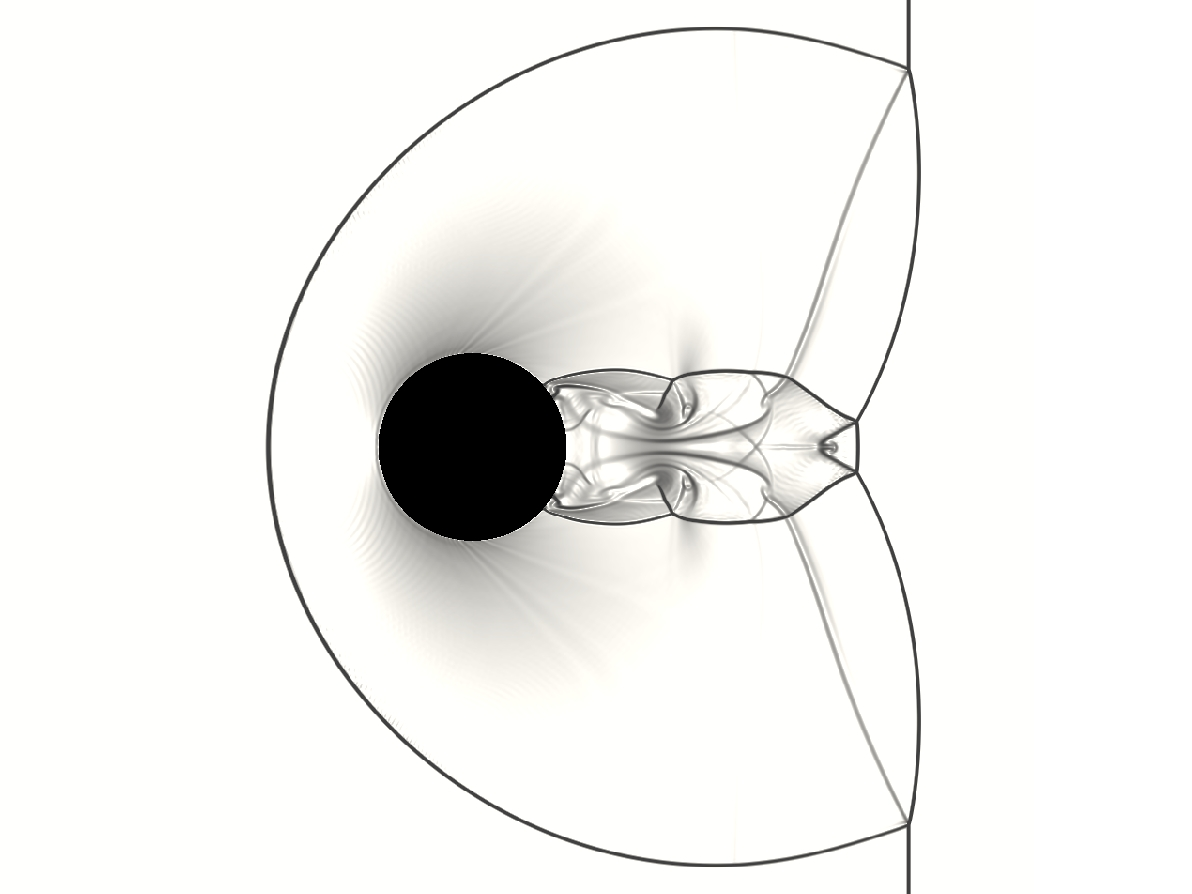
\includegraphics[trim = 30mm 0mm 30mm 0mm, clip, width=0.40\textwidth]{shock_cyn}
		\caption[激波圆柱作用]{激波圆柱作用。}
		\label{fig:shock_cyn}
	\end{figure}

	多图的插入如图~\ref{fig:oaspl},多图不应在子图中给文本子标题,只要给序号,并
	在主标题中进行引用说明。
	\begin{figure}[h]
		\centering
		\begin{subfigure}[b]{0.35\textwidth}
			\includegraphics[width=\textwidth]{oaspl_a}
			\caption{}
			\label{fig:oaspl_a}
		\end{subfigure}%
		~% add desired spacing
		\begin{subfigure}[b]{0.35\textwidth}
			\includegraphics[width=\textwidth]{oaspl_b}
			\caption{}
			\label{fig:oaspl_b}
		\end{subfigure}
		\begin{subfigure}[b]{0.35\textwidth}
			\includegraphics[width=\textwidth]{oaspl_c}
			\caption{}
			\label{fig:oaspl_c}
		\end{subfigure}%
		~% add desired spacing
		\begin{subfigure}[b]{0.35\textwidth}
			\includegraphics[width=\textwidth]{oaspl_d}
			\caption{}
			\label{fig:oaspl_d}
		\end{subfigure}
		\caption[总声压级]{总声压级。(a) 这是子图说明信息,(b) 这是子图说明信息,(c) 这是子图说明信息,(d) 这是子图说明信息。}
		\label{fig:oaspl}
	\end{figure}

	\subsection{算法}\label{sub:algorithms}

	算法环境在浙传毕设论文官方Word模板中未作明确要求,故暂采用通用样式,如算法
	\ref{alg:euclid}所示,详细使用方法请参见文档
	\href{https://ctan.org/pkg/algorithmicx?lang=en}{algorithmicx}。

	\begin{algorithm}[h]
		\small
		\caption{Euclid算法}\label{alg:euclid}
		\begin{algorithmic}[1]
			\Procedure{Euclid}{$a,b$}\Comment{$a$与$b$的最大公约数}
			\State $r\gets a\bmod b$
			\While{$r\not=0$}\Comment{若$r$为0则可跳出循环并返回答案}
			\State $a\gets b$
			\State $b\gets r$
			\State $r\gets a\bmod b$
			\EndWhile\label{euclidendwhile}
			\State \textbf{return} $b$\Comment{最大公约数为$b$}
			\EndProcedure
		\end{algorithmic}
	\end{algorithm}

	\subsection{代码段}\label{sub:listings}

	在正文中引用一段代码,可使用lstlisting设置代码环境。本模板的代码环境默认配置
	在artratex.sty,搜索关键字“\verb|\lstset|”即可找到相应配置。

	观察代码段~\ref{code:samp-code},结合前述图表设置,试图理解代码环境的编写。

	\begin{lstlisting}[
            language=C++,
            label=code:samp-code,
            caption=一段Chromium的源代码
        ]
        // Start tasks to take all the threads and block them.
        const int kNumBlockTasks = static_cast<int>(kNumWorkerThreads);
        for (int i = 0; i < kNumBlockTasks; ++i) {
            EXPECT_TRUE(pool()->PostWorkerTask(
                FROM_HERE,
                base::Bind(&TestTracker::BlockTask, tracker(), i, &blocker)));
        }
        tracker()->WaitUntilTasksBlocked(kNumWorkerThreads);

        // Setup to open the floodgates from within Shutdown().
        SetWillWaitForShutdownCallback(
            base::Bind(&TestTracker::PostBlockingTaskThenUnblockThreads,
                        scoped_refptr<TestTracker>(tracker()), pool(), &blocker,
                        kNumWorkerThreads));
        pool()->Shutdown(kNumWorkerThreads + 1);

        // Ensure that the correct number of tasks actually got run.
        tracker()->WaitUntilTasksComplete(static_cast<size_t>(kNumWorkerThreads + 1));
        tracker()->ClearCompleteSequence();
    \end{lstlisting}

	引用一两行代码,可以直接使用\texttt{verbatim}环境完成;若想调整环境中字体大
	小,可先用\verb|\begingroup|和\verb|\endgroup|将其包住,后加入字体大小命令。
	注意,此环境不会采取任何主动断行策略。

	\begingroup
	\small
	\begin{verbatim}
Error: Command failed: /bin/sh -c rsync -arvq --exclude cache
--exclude .git 
    \end{verbatim}
	\endgroup

	\begin{leftbar}
		\noindent\textbf{建议:}原则上,论文正文中应尽可能少出现工程代码片段,建
		议每段代码不超过一页(半页以内尤佳),并在正文中配有相应解释说明;超过一
		页的代码片段可拆分成多个模块(函数)分别列出并解释,若实在无法拆分,可将
		其放到附录中。
	\end{leftbar}

	\subsection{参考文献引用}\label{sub:references}

	参考文献引用过程以实例进行介绍,假设需要引用名为``Document Preparation
	System''的文献,步骤如下:
	\begin{enumerate}
		\item 使用Google Scholar搜索Document Preparation System,在目标条目下点
		      击Cite,展开后选择Import into BibTeX打开此文章的\hologo{BibTeX}索
		      引信息,将它们copy添加到references.bib文件中(此文件位于
		      bibliography文件夹下)。
		\item 索引第一行 \verb|@article{lamport1986document,|中
		      \verb|lamport1986document|即为此文献的label (\textbf{中文文献也必
			      须使用英文label},一般遵照:姓氏拼音+年份+标题第一字拼音的格式),
		      想要在论文中索引此文献,有两种索引类型:
		      \begin{itemize}
			      \item 文本类型:\verb|\citet{lamport1986document}|,正如此处所
			            示\citet{lamport1986document};
			      \item 括号类型:\verb|\citep{lamport1986document}|。正如此处所
			            示\citep{lamport1986document}。
		      \end{itemize}
		      \textbf{多文献索引用须用英文逗号隔开}:
		      \begin{itemize}
			      \item \verb|\citep{lamport1986document, chu2004tushu,
				            chen2005zhulu}|,正如此处所示\citep{lamport1986document,
				            chu2004tushu, chen2005zhulu}。
		      \end{itemize}
	\end{enumerate}

	更多例子如:\citet{walls2013drought}根据...的研究,首次提出...。其中关于
	...\citep{walls2013drought},是当前中国...得到迅速发展的研究领域
	\citep{chen1980zhongguo}。引用同一著者在同一年份出版的多篇文献时,在出版年份
	之后用英文小写字母区别,如:\citep{yuan2012lana, yuan2012lanb,
		yuan2012lanc}。同一处引用多篇文献时,按出版年份由近及远依次标注,中间用分号
	分开,例如\citep{chen1980zhongguo, stamerjohanns2009mathml, hls2012jinji,
		niu2013zonghe}。

	使用著者-出版年制(authoryear)式参考文献样式时,中文文献必须在
	\hologo{BibTeX}索引信息的\textbf{key} 域(请参考references.bib文件)填写作者
	姓名的拼音,才能使得文献列表按照拼音排序。参考文献表中的条目(不排序号),先
	按语种分类排列,语种顺序是:中文、日文、英文、俄文、其他文种。然后,中文按汉
	语拼音字母顺序排列,日文按第一著者的姓氏笔画排序,西文和 俄文按第一著者姓氏
	首字母顺序排列。如中\citep{niu2013zonghe}、日\citep{Bohan1928}、英
	\citep{stamerjohanns2009mathml}、俄\citep{Dubrovin1906}。

	不同文献样式和引用样式,如著者-出版年制(authoryear)、顺序编码制
	(numbers)、上标顺序编码制(super)可在cuzthesis.tex中修改调用artratex.sty
	的参数实现,如:
	\begin{itemize}
		\item \verb+\usepackage[numbers]{artratex}+ $\%$ 文本: Jones [1]; 括号: [1]
		\item \verb+\usepackage[super]{artratex}+ $\%$ 文本: Jones 上标[1]; 括号: 上标[1]
		\item \verb+\usepackage[authoryear]{artratex}+ $\%$ 文本: Jones (1995); 括号: (Jones, 1995)
		\item \verb+\usepackage[alpha]{artratex}+ $\%$ 文本: 不可用; 括号: [Jon95]
	\end{itemize}

	当前文档的默认参考文献样式为\textbf{super}。在该模式下,若希望在特定位置将上
	标改为嵌入式标,可使用:

	\begin{itemize}
		\item 文本类型:\verb|\citetns{lamport1986document,chen2005zhulu}|,正如此处
		      所示\citetns{lamport1986document,chen2005zhulu};
		\item 括号类型:\verb|\citepns{lamport1986document,chen2005zhulu}|;正如此处
		      所示\citepns{lamport1986document,chen2005zhulu}。
	\end{itemize}

	参考文献索引更为详细的信息,请见
	\href{https://github.com/zepinglee/gbt7714-bibtex-style}{zepinglee} 和
	\href{https://en.wikibooks.org/wiki/LaTeX/Bibliography_Management}{WiKibook
		Bibliography}。

	% \nocite{*}

	\section{常见使用问题}\label{sec:qa}

	\begin{itemize}
		\item 模板每次发布前,都已在Windows,Linux,macOS系统上测试通过。下载模
		      板后,若编译出现错误,则请参考国科大模板附带的
		      \href{https://github.com/mohuangrui/ucasthesis/wiki}{\LaTeX{}知识
			      小站} 中的
		      \href{https://github.com/mohuangrui/ucasthesis/wiki/%E7%BC%96%E8%AF%91%E6%8C%87%E5%8D%97}{编
			      译指南}。
		\item 模板文档的编码为UTF-8编码。所有文件都必须采用UTF-8编码,否则编译后
		      生成的文档将出现乱码文本。若出现文本编辑器无法打开文档或打开文档乱
		      码的问题,请检查编辑器对UTF-8编码的支持。
		\item 推荐选择\hologo{XeLaTeX}编译引擎编译中文文档。编译脚本的默认设定为
		      \hologo{XeLaTeX}编译引擎。你也可以选择不使用脚本编译,如直接使用
		      \LaTeX{}文本编辑器编译。注:\LaTeX{}文本编辑器编译的默认设定为
		      \hologo{pdfLaTeX}编译引擎,若选择\hologo{XeLaTeX}编译引擎,请进入
		      下拉菜单选择。为正确生成引用链接,需要进行全编译。由于
		      \hologo{LuaLaTeX}编译引擎尚不成熟,故暂不推荐。
		\item VS Code中关于\hologo{LaTeX}方面建议安装的插件:
		      \begin{itemize}
			      \item \hologo{LaTeX} Workshop:提供了绝大多数\hologo{LaTeX}的
			            辅助功能;
			      \item Rewrap:可使用\verb|Alt+Q|进行硬换行(即自动重排段落使得
			            每行不超过指定宽度)。
		      \end{itemize}
		      其他一些有用的插件有:
		      \begin{itemize}
			      \item Git Graph;以更形象的方式查看Git提交记录,并可做出一些简
			            单Git操作;
			      \item gitignore:对.gitignore文件进行操作;
			      \item Markdown Preview Enhanced:提供了Markdown语法支持与预
			            览。
		      \end{itemize}
		\item 设置文档样式: 在artratex.sty中搜索关键字定位相应命令,然后修改:
		      \begin{itemize}
			      \item 正文行距:启用和设置 \verb|\linespread{1.5}|,默认1.5倍
			            行距。
			      \item 参考文献行距:修改 \verb|\setlength{\bibsep}{0.0ex}|
			      \item 目录显示级数:修改 \verb|\setcounter{tocdepth}{2}|
			      \item 文档超链接的颜色及其显示:修改 \verb|\hypersetup|
		      \end{itemize}
		\item 文档内字体切换方法:
		      \begin{itemize}
			      \item 宋体:浙传论文模板cuzthesis 或 \textrm{浙传论文模板
				            cuzthesis}
			      \item 粗宋体:{\bfseries 浙传论文模板cuzthesis} 或 \textbf{浙
				            传论文模板cuzthesis}
			      \item 黑体:{\sffamily 浙传论文模板cuzthesis} 或 \textsf{浙传
				            论文模板cuzthesis}
			      \item 粗黑体:{\bfseries\sffamily 浙传论文模板cuzthesis} 或
			            \textsf{\bfseries 浙传论文模板cuzthesis}
			      \item 仿宋:{\ttfamily 浙传论文模板cuzthesis} 或 \texttt{浙传
				            论文模板cuzthesis}
			      \item 粗仿宋:{\bfseries\ttfamily 浙传论文模板cuzthesis} 或
			            \texttt{\bfseries 浙传论文模板cuzthesis}
			      \item 楷体:{\itshape 浙传论文模板cuzthesis} 或 \textit{浙传论
				            文模板cuzthesis}
			      \item 粗楷体:{\bfseries\itshape 浙传论文模板cuzthesis} 或
			            \textit{\bfseries 浙传论文模板cuzthesis}
		      \end{itemize}
	\end{itemize}

\end{cuzchapter}
% Guidance
% \chapter{总结与展望}\label{chap:conclusions}
\begin{cuzchapter}{总结与展望}{chap:conclusions}

	本文主要介绍了浙传\hologo{LaTeX}模板cuzthesis的一些基本用法与注意事项,同时
	也对论文各部分的写法做了简要说明并提出了一些意见与建议。相信读者通过阅读本文
	档,当可对浙传毕业论文的撰写(包括内容与格式)有一个大概认识。

	诚然,不足之处在所难免:模板类中一些设计尚存在不甚合理之处,适用情况亦不够普
	遍。但相信随着\hologo{LaTeX}知识的增长,上述缺憾可逐一弥补。

	\begin{leftbar}
		\noindent\textbf{建议:}该部分应对全文做出总结与概括,抓住重点、简明扼
		要;在此基础上,列出不足之处,并简要提出可能的改进想法与未来展望。
	\end{leftbar}

\end{cuzchapter}% Conclusions
%---------------------------------------------------------------------------%
%
%-
%-> Backmatter: acknowledgement, references, appendices (if any)
%-
%-> The references
\intotoc{\bibname}% add link to contents table and bookmark
% \begingroup
% \linespread{1.2}\selectfont
\bibliography{bibliography/references}%
% \endgroup
%-> The acknowledgement
\begin{acknowledgement}
	感谢ucasthesis模板作者莫晃锐!感谢所有\hologo{LaTeX}社区的各位无名英雄!感谢
	Google搜索引擎!感谢所有帮助过我的人!若无上述帮助与参考,我无法完成此模板的
	制作。当然此模板尚有许多不足之处,然可在后面不断完善。最后,再次对上述人士表
	示衷心感谢!
	
	\begin{leftbar}
		\noindent\textbf{建议:}该部分一般需要感谢四部分人:老师、父母、同学与朋
		友,可简要陈述所受之帮助。仅可在此处抒发情感,但文字不宜过多,一页即可;
		亦不可过少,免显薄情寡义。
	\end{leftbar}
\end{acknowledgement}%
%-> The appendices (if any)
\appendix% change the page layout
% \chapter{中国科学院大学学位论文撰写要求}
\begin{appendices}\label{sec:appendices}

	\section*{论文无附录者无需附录部分}

	\section*{测试公式编号} \label{sec:testmath}

	参见式\eqref{eq:appedns}与式\eqref{eq:2}:

	\begin{equation} \label{eq:appedns}
		\begin{cases}
			\frac{\partial \rho}{\partial t} + \nabla\cdot(\rho\Vector{V}) = 0 \ \mathrm{times\ font\ test}                                            \\
			\frac{\partial (\rho\Vector{V})}{\partial t} + \nabla\cdot(\rho\Vector{V}\Vector{V}) = \nabla\cdot\Tensor{\sigma} \ \text{times font test} \\
			\frac{\partial (\rho E)}{\partial t} + \nabla\cdot(\rho E\Vector{V}) = \nabla\cdot(k\nabla T) + \nabla\cdot(\Tensor{\sigma}\cdot\Vector{V})
		\end{cases}
	\end{equation}
	\begin{equation} \label{eq:2}
		\frac{\partial }{\partial t}\int\limits_{\Omega} u \, \mathrm{d}\Omega + \int\limits_{S} \unitVector{n}\cdot(u\Vector{V}) \, \mathrm{d}S = \dot{\phi}
	\end{equation}

	\section*{测试代码段编号} \label{sec:testlistings}

	参见代码段
	\ref{code:samp-code-c}、\ref{code:samp-code-cpp}、\ref{code:samp-code-java}、\ref{code:samp-code-csharp}、
	\ref{code:samp-code-python}与\ref{code:samp-code-latex}:

    \begin{listing}[H]
        \centering
        \caption{一段简单得不能再简单的C代码}
        \label{code:samp-code-c}
        \begin{ccode}
            /* 一段简单得不能再简单的C代码 */
            #include <stdio.h>

            int main(int argc, char const **argv) {
                printf("Hello CUZThesis!!\n");
                return 0;
            }
        \end{ccode}
    \end{listing}

    \begin{listing}[H]
        \centering
        \caption{一段简单得不能再简单的C++代码}
        \label{code:samp-code-cpp}
        \begin{cppcode}
            /* 一段简单得不能再简单的C++代码 */
            #include <iostream>

            int main(int argc, char const **argv) {
                std::cout << "Hello CUZThesis!!" << std::endl;
                return 0;
            }
        \end{cppcode}   
    \end{listing}

    \begin{listing}[H]
        \centering
        \caption{一段简单得不能再简单的Java代码}
        \label{code:samp-code-java}
        \begin{javacode}
            // 一段简单得不能再简单的Java代码
            class HelloCUZThesis {
                public static void main(String[] args) {
                    System.out.println("Hello CUZThesis!!");
                }
            }
        \end{javacode}
    \end{listing}

    \begin{listing}[H]
        \centering
        \caption{一段简单得不能再简单的C\#代码}
        \label{code:samp-code-csharp}
        \begin{csharpcode}
            // 一段简单得不能再简单的C#代码
            class HelloCUZThesis {
                public static void Main(string[] args) {
                    Console.WriteLine("Hello CUZThesis!!");
                }
            }
        \end{csharpcode}
    \end{listing}

    \begin{listing}[H]
        \centering
        \caption{一段简单得不能再简单的Python代码}
        \label{code:samp-code-python}
        \begin{pythoncode}
            # 一段简单得不能再简单的Python代码
            print("Hello CUZThesis!!")
        \end{pythoncode}
    \end{listing}

    \begin{listing}[H]
        \centering
        \caption{一段简单得不能再简单的\hologo{LaTeX}代码}
        \label{code:samp-code-latex}
        \begin{texcode}
            % 一段简单得不能再简单的\hologo{LaTeX}代码
            \documentclass{article}

            \begin{document}    
                Hello CUZThesis!!
            \end{document}
        \end{texcode}
    \end{listing}

	\section*{测试生僻字} \label{sec:testcharacters}

	霜蟾盥薇曜灵霜颸妙鬘虚霩淩澌菀枯菡萏泬寥窅冥毰毸濩落霅霅便嬛岧峣瀺灂姽婳愔嫕
	飒纚棽俪緸冤莩甲摛藻卮言倥侗椒觞期颐夜阑彬蔚倥偬澄廓簪缨陟遐迤逦缥缃鹣鲽憯懔
	闺闼璀错媕婀噌吰澒洞阛闠覼缕玓瓑逡巡諓諓琭琭瀌瀌踽踽叆叇氤氲瓠犀流眄蹀躞赟嬛
	茕頔璎珞螓首蘅皋惏悷缱绻昶皴皱颟顸愀然菡萏卑陬纯懿犇麤掱暒墌墍墎墏墐墒墒墓墔
	墕墖墘墖墚墛坠墝增墠墡墢墣墤墥墦墧墨墩墪樽墬墭堕墯墰墱墲坟墴墵垯墷墸墹墺墙墼
	墽垦墿壀壁壂壃壄壅壆坛壈壉壊垱壌壍埙壏壐壑壒压壔壕壖壗垒圹垆壛壜壝垄壠壡坜壣
	壤壥壦壧壨坝塆圭嫶嫷嫸嫹嫺娴嫼嫽嫾婳妫嬁嬂嬃嬄嬅嬆嬇娆嬉嬊娇嬍嬎嬏嬐嬑嬒嬓嬔
	嬕嬖嬗嬘嫱嬚嬛嬜嬞嬟嬠嫒嬢嬣嬥嬦嬧嬨嬩嫔嬫嬬奶嬬嬮嬯婴嬱嬲嬳嬴嬵嬶嬷婶嬹嬺嬻
	嬼嬽嬾嬿孀孁孂娘孄孅孆孇孆孈孉孊娈孋孊孍孎孏嫫婿媚嵭嵮嵯嵰嵱嵲嵳嵴嵵嵶嵷嵸嵹
	嵺嵻嵼嵽嵾嵿嶀嵝嶂嶃崭嶅嶆岖嶈嶉嶊嶋嶌嶍嶎嶏嶐嶑嶒嶓嵚嶕嶖嶘嶙嶚嶛嶜嶝嶞嶟峤
	嶡峣嶣嶤嶥嶦峄峃嶩嶪嶫嶬嶭崄嶯嶰嶱嶲嶳岙嶵嶶嶷嵘嶹岭嶻屿岳帋巀巁巂巃巄巅巆巇
	巈巉巊岿巌巍巎巏巐巑峦巓巅巕岩巗巘巙巚帠帡帢帣帤帨帩帪帬帯帰帱帲帴帵帷帹帺帻
	帼帽帾帿幁幂帏幄幅幆幇幈幉幊幋幌幍幎幏幐幑幒幓幖幙幚幛幜幝幞帜幠幡幢幤幥幦幧
	幨幩幪幭幮幯幰幱庍庎庑庖庘庛庝庠庡庢庣庤庥庨庩庪庬庮庯庰庱庲庳庴庵庹庺庻庼庽
	庿廀厕廃厩廅廆廇廋廌廍庼廏廐廑廒廔廕廖廗廘廙廛廜廞庑廤廥廦廧廨廭廮廯廰痈廲廵
	廸廹廻廼廽廿弁弅弆弇弉弖弙弚弜弝弞弡弢弣弤弨弩弪弫弬弭弮弰弲弪弴弶弸弻弼弽弿
	彖彗彘彚彛彜彝彞彟彴彵彶彷彸役彺彻彽彾佛徂徃徆徇徉后徍徎徏径徒従徔徕徖徙徚徛
	徜徝从徟徕御徢徣徤徥徦徧徨复循徫旁徭微徯徰徱徲徳徴徵徶德徸彻徺忁忂惔愔忇忈忉
	忔忕忖忚忛応忝忞忟忪挣挦挧挨挩挪挫挬挭挮挰掇授掉掊掋掍掎掐掑排掓掔掕挜掚挂掜
	掝掞掟掠采探掣掤掦措掫掬掭掮掯掰掱掲掳掴掵掶掸掹掺掻掼掽掾掿拣揁揂揃揅揄揆揇
	揈揉揊揋揌揍揎揑揓揔揕揖揗揘揙揤揥揦揧揨揫捂揰揱揲揳援揵揶揷揸揻揼揾揿搀搁搂
	搃搄搅搇搈搉搊搋搌搎搏搐搑搒摓摔摕摖摗摙摚摛掼摝摞摠摡斫斩斮斱斲斳斴斵斶斸旪
	旫旮旯晒晓晔晕晖晗晘晙晛晜晞晟晠晡晰晣晤晥晦晧晪晫晬晭晰晱晲晳晴晵晷晸晹晻晼
	晽晾晿暀暁暂暃暄暅暆暇晕晖暊暋暌暍暎暏暐暑暒暓暔暕暖暗旸暙暚暛暜暝暞暟暠暡暣
	暤暥暦暧暨暩暪暬暭暮暯暰昵暲暳暴暵暶暷暸暹暺暻暼暽暾暿曀曁曂曃晔曅曈曊曋曌曍
	曎曏曐曑曒曓曔曕曗曘曙曚曛曜曝曞曟旷曡曢曣曤曥曦曧昽曩曪曫晒曭曮曯椗椘椙椚椛
	検椝椞椟椠椡椢椣椤椥椦椧椨椩椪椫椬椭椮椯椰椱椲椳椴椵椶椷椸椹椺椻椼椽椾椿楀楁
	楂楃楅楆楇楈楉杨楋楌楍榴榵榶榷榸榹榺榻榼榽榾桤槀槁槂盘槄槅槆槇槈槉槊构槌枪槎
	槏槐槑槒杠槔槕槖槗滙滛滜滝滞滟滠滢滣滦滧滪滫沪滭滮滰滱渗滳滵滶滹滺浐滼滽漀漃
	漄漅漈漉溇漋漌漍漎漐漑澙熹漗漘漙沤漛漜漝漞漟漡漤漥漦漧漨漪渍漭漮漯漰漱漳漴溆
	漶漷漹漺漻漼漽漾浆潀颍潂潃潄潅潆潇潈潉潊潋潌潍潎潏潐潒潓洁潕潖潗潘沩潚潜潝潞
	潟潠潡潢潣润潥潦潧潨潩潪潫潬潭浔溃潱潲潳潴潵潶滗潸潹潺潻潼潽潾涠澁澄澃澅浇涝
	澈澉澊澋澌澍澎澏湃澐澑澒澓澔澕澖涧澘澙澚澛澜澝澞澟渑澢澣泽浍澯澰淀澲澳澴澵澶
	澷澸潇潆瀡瀢瀣瀤瀥潴泷濑瀩瀪瀫瀬瀭瀮瀯弥瀱潋瀳瀴瀵瀶瀷瀸瀹瀺瀻瀼瀽澜瀿灀灁瀺
	灂沣滠灅灆灇灈灉灊灋灌灍灎灏灐洒灒灓漓灖灗滩灙灚灛灜灏灞灟灠灡灢湾滦灥灦灧灨
	灪燝燞燠燡燢燣燤燥灿燧燨燩燪燫燮燯燰燱燲燳烩燵燵燸燹燺薰燽焘燿爀爁爂爃爄爅爇
	爈爉爊爋爌烁爎爏爑爒爓爔爕爖爗爘爙爚烂爜爝爞爟爠爡爢爣爤爥爦爧爨爩猽猾獀犸獂
	獆獇獈獉獊獋獌獍獏獐獑獒獓獔獕獖獗獘獙獚獛獜獝獞獟獠獡獢獣獤獥獦獧獩狯猃獬獭
	狝獯狞獱獳獴獶獹獽獾獿猡玁玂玃。

	\begin{leftbar}
		\noindent\textbf{建议:}附录为可选部分,一般用来存放不适合在正文中列出的
		大段内容,如较长的表格、代码段等。若需分小节列出,则应采用加星号版本的小
		节命令\verb|\section*{}|,以避免出现不正确的章节号。
	\end{leftbar}

\end{appendices}%
\end{document}
%---------------------------------------------------------------------------%

